\begin{document}
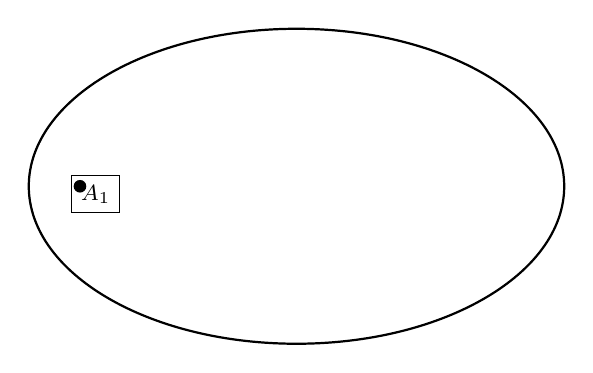
\begin{tikzpicture}[
  scale=1.0,
  >=stealth,
  every node/.style={font=\small},
  box/.style={draw, font={\sffamily\footnotesize}}
]
  \def\a{3.4}
  \def\b{2.0}
  \pgfmathsetmacro{\c}{sqrt(\a*\a-\b*\b)}
  \draw[thick] (0,0) ellipse [x radius=\a, y radius=\b];
  \fill (-\c,0) circle (0.08);
  \node[box] at (-\c+0.2,-0.10) {$A_1$};
  \draw plot[domain=140:200, samples=20]
    ({\a*cos(\x)},{\b*sin(\x)});
\end{tikzpicture}
\end{document}
